\chapter{METHODOLOGY}

\section{Pipeline overview}

The plugin runs seven stages per detected hole. Stage~4 is the algorithmic core; the others prepare the patch for it or clean up after it. Stages~5 and~6 must run in this order: uniform Laplacian smoothing applied after displacement would erase the dome that displacement creates, because uniform smoothing exhibits shrinkage on curved surfaces.

This ordering was reversed in an early version of the implementation. Stage~6 produced patches with localised spike artifacts, and applying Stage~5 afterwards seemed like a natural cleanup pass --- right up until the result on \texttt{sphere\_large} was overlaid on the ground truth and the dome turned out to have been quietly flattened. Reordering the two stages and using Taubin (which preserves low frequencies) in Stage~6 for spike cleanup fixed both problems at once.

\begin{figure}[H]
    \centering
    \begin{tikzpicture}[
        node distance=0.5cm,
        stage/.style={rectangle, rounded corners=4pt, draw=ackblue!70, thick,
                      fill=ackblue!8, minimum width=8.5cm, minimum height=0.8cm,
                      align=center, font=\small},
        core/.style={rectangle, rounded corners=4pt, draw=red!70, very thick,
                     fill=red!10, minimum width=8.5cm, minimum height=0.95cm,
                     align=center, font=\small\bfseries},
        io/.style={rectangle, draw=black!60, dashed,
                   minimum width=8.5cm, minimum height=0.65cm, align=center,
                   font=\small\itshape},
        arrow/.style={-{Stealth[length=2mm]}, thick}
    ]
        \node[io] (in) {Input mesh with hole(s)};
        \node[stage, below=of in] (s1) {1. Hole detection};
        \node[stage, below=of s1] (s2) {2. Boundary analysis};
        \node[stage, below=of s2] (s3) {3. Initial triangulation};
        \node[core,  below=of s3] (s4) {4. Normal field diffusion (core)};
        \node[stage, below=of s4] (s5) {5. Laplacian smoothing};
        \node[stage, below=of s5] (s6) {6. Curvature-guided displacement + Taubin};
        \node[stage, below=of s6] (s7) {7. Patch merge};
        \node[io,    below=of s7] (out) {Output: filled mesh};
        \draw[arrow] (in) -- (s1);
        \draw[arrow] (s1) -- (s2);
        \draw[arrow] (s2) -- (s3);
        \draw[arrow] (s3) -- (s4);
        \draw[arrow] (s4) -- (s5);
        \draw[arrow] (s5) -- (s6);
        \draw[arrow] (s6) -- (s7);
        \draw[arrow] (s7) -- (out);
    \end{tikzpicture}
    \caption{The seven-stage pipeline.}
    \label{fig:pipeline}
\end{figure}

\section{Hole detection}

VCGlib's adjacency machinery does most of the work. After enabling face--face and vertex--face adjacency and calling \texttt{UpdateFlags::FaceBorderFromFF}, each border edge has its flag set, and we walk the boundary by hopping from one border edge to the next using \texttt{VFIterator}. In a 2-manifold mesh each boundary vertex has exactly two incident border edges, so excluding the previous vertex uniquely determines the next one.

\begin{algorithm}[H]
\caption{Boundary loop walk}
\begin{algorithmic}[1]
\For{each face $f$, each local edge $e$}
    \If{$\texttt{IsBorder}(f, e)$ and edge unvisited}
        \State $\text{start} \gets V_e$;\ $\text{curr} \gets V_e$;\ $\text{next} \gets V_{e+1}$
        \While{$\text{curr} \ne \text{start}$ on subsequent iterations}
            \State append \text{curr}; mark $(\text{curr}, \text{next})$ visited
            \State $\text{prev} \gets \text{curr}$;\ $\text{curr} \gets \text{next}$
            \State find next border edge $(\text{curr}, x)$ with $x \ne \text{prev}$
            \State $\text{next} \gets x$
        \EndWhile
    \EndIf
\EndFor
\end{algorithmic}
\end{algorithm}

A safety counter and a length sanity check on the loop guard against non-manifold input. Holes longer than \texttt{MaxHoleSize} edges are skipped so the user can opt in.

\section{Boundary analysis}

For each boundary vertex, the area-weighted normal is read from \texttt{vp->N()} (cached by VCG after the topology update) and the mean curvature is computed from the cotangent Laplacian. The cotangent of an angle is evaluated as
\begin{equation}
\cot \theta = \frac{\vec{AB} \cdot \vec{AC}}{\|\vec{AB} \times \vec{AC}\|},
\end{equation}
which avoids calls to \texttt{acos} and \texttt{sin} and remains numerically stable near 0 and $\pi$. Weights accumulate face by face: in face $(v_i, v_B, v_C)$, the angle at $C$ contributes to $w_{iB}$ and the angle at $B$ contributes to $w_{iC}$. Each interior edge collects contributions from both adjacent faces; border edges receive only one, which matches the formula on an open surface.

The resulting mean curvature $H_i = \|L_{\text{cot}}\|/(2 \sum_j w_{ij})$ is stored but not used downstream. The displacement step in Stage~6 estimates dome height from boundary normal angles directly, so $H_i$ is kept only as a sanity-check value during debugging.

\section{Initial triangulation}

The patch is built in four sub-steps: project to 2D, ear-clip, Delaunay-flip, refine.

\subsection*{2D projection}

Compute the average boundary normal $\bar{\mathbf{n}}$ and pick two perpendicular axes $(\mathbf{u}, \mathbf{v})$ to form a tangent frame. Project each boundary vertex by subtracting the centroid and dotting with $\mathbf{u}, \mathbf{v}$. The signed area via the shoelace formula tells us whether the projected polygon is CCW; if not, we reverse it.

\begin{figure}[H]
    \centering
    \begin{tikzpicture}[scale=0.95, line join=round, line cap=round]
        \pgfmathsetmacro{\sx}{0.7}
        \pgfmathsetmacro{\sy}{0.35}
        \coordinate (A) at (-3.0, 0);
        \coordinate (B) at ( 3.0, 0);
        \coordinate (C) at ($(B) + (\sx*3, \sy*3)$);
        \coordinate (D) at ($(A) + (\sx*3, \sy*3)$);
        \fill[ackblue!6] (A) -- (B) -- (C) -- (D) -- cycle;
        \draw[gray!55, dashed] (A) -- (B) -- (C) -- (D) -- cycle;
        \node[gray!70, font=\footnotesize, right=1pt] at (C) {tangent plane};
        \coordinate (c) at ($0.5*(A) + 0.5*(C)$);
        \fill[red] (c) circle (2pt);
        \node[red, font=\small, below left=-1pt] at (c) {$c_{\partial}$};
        \draw[-{Stealth[length=3mm]}, very thick, red] (c) -- ++(0, 2.4);
        \node[red, font=\small, right] at ($(c) + (0, 2.0)$) {$\bar{\mathbf{n}}$};
        \foreach \i/\ang/\dz in {0/30/0.55, 1/90/0.30, 2/150/0.70, 3/210/0.25, 4/270/0.60, 5/330/0.35} {
            \pgfmathsetmacro{\ang}{60*\i + 30}
            \coordinate (p\i) at ($(c) + ({1.5*cos(\ang)}, {0.8*sin(\ang)})$);
            \coordinate (v\i) at ($(p\i) + (0, {1.1 + \dz})$);
        }
        \foreach \i in {0,...,5} {
            \draw[dotted, gray!70] (v\i) -- (p\i);
        }
        \draw[very thick, blue!75!black]
            (v0) -- (v1) -- (v2) -- (v3) -- (v4) -- (v5) -- cycle;
        \foreach \i in {0,...,5} { \fill[blue!75!black] (v\i) circle (2pt); }
        \draw[thick, orange!90!black]
            (p0) -- (p1) -- (p2) -- (p3) -- (p4) -- (p5) -- cycle;
        \foreach \i in {0,...,5} { \fill[orange!90!black] (p\i) circle (1.6pt); }
    \end{tikzpicture}
    \caption{Projection of the 3D boundary (blue) onto the tangent plane defined by $\bar{\mathbf{n}}$.}
    \label{fig:2d-projection}
\end{figure}

\subsection*{Ear clipping}

The naive version of ear clipping picks the first valid ear at each step, which on a regular polygon degenerates into a fan of sliver triangles (Figure~\ref{fig:ear-clipping}, left). The implementation scans every valid ear at each step and picks the one whose minimum interior angle is largest. This produces a noticeably more even tessellation. Three fallback layers handle pathological input: if no valid ear exists, the first convex vertex is clipped; if no convex vertex exists, vertex 1 is force-clipped; if the polygon collapses below three vertices, the loop stops. A winding check against $\bar{\mathbf{n}}$ at the end flips the triangle ordering if the patch ended up facing the wrong way.

The first version of this stage used FIFO ear selection. The patch on \texttt{sphere\_small} came out as a fan of slivers concentrated at one vertex, and downstream this caused Stage~4 to produce visibly biased normals near that vertex. Switching the heuristic to max-min interior angle was a five-line change and removed the bias.

\begin{figure}[H]
    \centering
    \begin{tikzpicture}[scale=0.85, line join=round]
        \begin{scope}[xshift=0cm]
            \node[font=\small\bfseries] at (0, 2.8) {FIFO (slivers)};
            \foreach \i/\lbl in {0/p_0, 1/p_1, 2/p_2, 3/p_3, 4/p_4, 5/p_5, 6/p_6, 7/p_7} {
                \coordinate (fan\i) at ({360/8 * \i + 90}:2);
            }
            \draw[thick, ackblue]
                (fan0) -- (fan1) -- (fan2) -- (fan3) -- (fan4) --
                (fan5) -- (fan6) -- (fan7) -- cycle;
            \foreach \i in {1,2,3,4,5,6} { \draw[red, thin] (fan0) -- (fan\i); }
            \foreach \i in {0,...,7} { \fill (fan\i) circle (1.5pt); }
        \end{scope}
        \begin{scope}[xshift=6.5cm]
            \node[font=\small\bfseries] at (0, 2.8) {Best-ear (regular)};
            \foreach \i in {0,...,7} { \coordinate (be\i) at ({360/8 * \i + 90}:2); }
            \draw[thick, ackblue]
                (be0) -- (be1) -- (be2) -- (be3) -- (be4) --
                (be5) -- (be6) -- (be7) -- cycle;
            \draw[green!50!black, thin] (be0) -- (be2);
            \draw[green!50!black, thin] (be2) -- (be4);
            \draw[green!50!black, thin] (be4) -- (be6);
            \draw[green!50!black, thin] (be6) -- (be0);
            \draw[green!50!black, thin] (be0) -- (be4);
            \foreach \i in {0,...,7} { \fill (be\i) circle (1.5pt); }
        \end{scope}
    \end{tikzpicture}
    \caption{FIFO ear clipping (left) versus best-ear clipping (right) on the same polygon.}
    \label{fig:ear-clipping}
\end{figure}

\subsection*{Delaunay flips and centroid refinement}

For each interior edge shared by two triangles, the alternate diagonal is considered as a flip candidate. The flip is accepted only if it strictly increases the minimum interior angle across the pair. A face that has already been flipped in the current pass is locked until the next one, which prevents conflicting flips during a single sweep. On the test meshes, three passes are enough to converge.

The flip pass was the part of Stage~3 that took longest to get right. The issue was deriving the correct winding for the new diagonal on a curved 3D patch: a global sign-check against $\bar{\mathbf{n}}$ works for nearly planar patches but breaks once the patch curves enough that the new triangle faces the opposite side of $\bar{\mathbf{n}}$ from the original. After being stuck on this for an hour or two, going back to the lecture material on mesh orientation gave the right hint --- the cyclic order of $u, v$ inside the original triangle $t_1$ already encodes the orientation locally, so no global vector is needed. The two-case split in the code (whether $t_1$ contains $u \to v$ or $v \to u$) is the consequence.

\begin{figure}[H]
    \centering
    \begin{tikzpicture}[scale=0.95, line join=round]
        \begin{scope}[xshift=0cm]
            \node[font=\small\bfseries] at (1.5, 3.1) {Before flip};
            \coordinate (u) at (0, 1.5); \coordinate (v) at (3, 1.5);
            \coordinate (w) at (1.5, 2.6); \coordinate (x) at (1.5, 0.4);
            \fill[ackblue!8] (u) -- (v) -- (w) -- cycle;
            \fill[ackblue!8] (u) -- (v) -- (x) -- cycle;
            \draw[thick] (u) -- (w) -- (v) -- (x) -- cycle;
            \draw[red, very thick] (u) -- (v);
            \fill (u) circle (1.6pt); \node[left]  at (u) {$u$};
            \fill (v) circle (1.6pt); \node[right] at (v) {$v$};
            \fill (w) circle (1.6pt); \node[above] at (w) {$w$};
            \fill (x) circle (1.6pt); \node[below] at (x) {$x$};
        \end{scope}
        \draw[-{Stealth[length=3mm]}, very thick]
            (3.8, 1.5) -- (4.8, 1.5) node[midway, above, font=\small] {flip};
        \begin{scope}[xshift=5.3cm]
            \node[font=\small\bfseries] at (1.5, 3.1) {After flip};
            \coordinate (u) at (0, 1.5); \coordinate (v) at (3, 1.5);
            \coordinate (w) at (1.5, 2.6); \coordinate (x) at (1.5, 0.4);
            \fill[green!8] (u) -- (w) -- (x) -- cycle;
            \fill[green!8] (v) -- (w) -- (x) -- cycle;
            \draw[thick] (u) -- (w) -- (v) -- (x) -- cycle;
            \draw[green!50!black, very thick] (w) -- (x);
            \fill (u) circle (1.6pt); \node[left]  at (u) {$u$};
            \fill (v) circle (1.6pt); \node[right] at (v) {$v$};
            \fill (w) circle (1.6pt); \node[above] at (w) {$w$};
            \fill (x) circle (1.6pt); \node[below] at (x) {$x$};
        \end{scope}
    \end{tikzpicture}
    \caption{Edge flip replaces diagonal $(u,v)$ with $(w,x)$ when this increases the minimum angle.}
    \label{fig:delaunay-flip}
\end{figure}

The target triangle area is set to that of an equilateral triangle with side $\bar{e} \cdot \texttt{RefinementFactor}$, where $\bar{e}$ is the average boundary edge length. Faces with area above $1.5 \times$ the target are split by inserting their centroid as a new interior vertex. Up to eight refinement passes run, capped at 200\,000 faces total to prevent runaway subdivision on aggressive parameter values. A second Delaunay flip pass cleans up slivers introduced by centroid insertion.

\section{Normal field diffusion}

This is the stage that gives the patch its curvature. Each component of the vertex normal is treated as a scalar field on the patch, the boundary values are pinned to those from Stage~2, and the heat equation is used to propagate boundary information inward. The continuous problem is
\begin{equation}
\frac{\partial \mathbf{n}}{\partial t} = \lambda \, \Delta_\Omega \mathbf{n}, \qquad \mathbf{n}\big|_{\partial\Omega} = \mathbf{n}^{\text{fixed}},
\end{equation}
applied component-wise. The steady state is the harmonic extension of the boundary normals into the patch interior.

\begin{figure}[H]
    \centering
    \begin{tikzpicture}[scale=0.85, line join=round, line cap=round]
        \pgfmathsetmacro{\R}{1.6}
        \tikzset{bnd/.style={-{Stealth[length=1.5mm]}, red, thick}}
        \tikzset{intarr/.style={-{Stealth[length=1.3mm]}, blue!70!black, thick}}
        \begin{scope}[xshift=0cm]
            \draw[thick, ackblue, fill=ackblue!4] (0, 0) circle (\R);
            \foreach \ang in {0, 30, 60, 90, 120, 150, 180, 210, 240, 270, 300, 330} {
                \draw[bnd] ({\R*cos(\ang)}, {\R*sin(\ang)})
                        -- ({(\R+0.55)*cos(\ang)}, {(\R+0.55)*sin(\ang)});
            }
            \node[gray!70, font=\footnotesize, align=center] at (0, 0) {interior\\unset};
            \node[font=\small\bfseries] at (0, -\R - 0.55) {$t = 0$};
        \end{scope}
        \begin{scope}[xshift=5.2cm]
            \draw[thick, ackblue, fill=ackblue!4] (0, 0) circle (\R);
            \foreach \ang in {0, 30, 60, 90, 120, 150, 180, 210, 240, 270, 300, 330} {
                \draw[bnd] ({\R*cos(\ang)}, {\R*sin(\ang)})
                        -- ({(\R+0.55)*cos(\ang)}, {(\R+0.55)*sin(\ang)});
            }
            \foreach \ang in {0, 60, 120, 180, 240, 300} {
                \draw[intarr] ({0.95*cos(\ang)}, {0.95*sin(\ang)})
                           -- ({(0.95+0.45)*cos(\ang)}, {(0.95+0.45)*sin(\ang)});
            }
            \node[font=\small\bfseries] at (0, -\R - 0.55) {$t = t_{\text{mid}}$};
        \end{scope}
        \begin{scope}[xshift=10.4cm]
            \draw[thick, ackblue, fill=ackblue!4] (0, 0) circle (\R);
            \foreach \ang in {0, 30, 60, 90, 120, 150, 180, 210, 240, 270, 300, 330} {
                \draw[bnd] ({\R*cos(\ang)}, {\R*sin(\ang)})
                        -- ({(\R+0.55)*cos(\ang)}, {(\R+0.55)*sin(\ang)});
            }
            \foreach \r in {0.55, 1.1} {
                \foreach \ang in {0, 45, 90, 135, 180, 225, 270, 315} {
                    \draw[intarr] ({\r*cos(\ang)}, {\r*sin(\ang)})
                               -- ({(\r+0.40)*cos(\ang)}, {(\r+0.40)*sin(\ang)});
                }
            }
            \node[font=\small\bfseries] at (0, -\R - 0.55) {$t \to \infty$};
        \end{scope}
        \draw[-{Stealth[length=3mm]}, thick] (2.3, 0) -- (2.9, 0);
        \draw[-{Stealth[length=3mm]}, thick] (7.5, 0) -- (8.1, 0);
    \end{tikzpicture}
    \caption{Heat-equation diffusion of the normal field, from initial state to harmonic steady state.}
    \label{fig:heat-diffusion}
\end{figure}

Discretising with implicit Euler gives, per component,
\begin{equation}
(I + \lambda L_{\text{cot}})\, \mathbf{n}^{t+1}_{\text{int}} = \mathbf{n}^{t}_{\text{int}} + \lambda\, \mathbf{b},
\end{equation}
where $\mathbf{b}_i = \sum_{j \in \partial \cap \mathcal{N}(i)} w_{ij}\, n_j^{\text{fixed}}$ collects the contributions from fixed boundary neighbours. This is the standard finite-element treatment of Dirichlet conditions: boundary values are eliminated from the unknown vector and reappear on the right-hand side. The system matrix is built from cotangent weights, computed face by face on the patch. Diagonal entries are $1 + \lambda \sum_j w_{ij}$, summing over \emph{all} neighbours (both interior and boundary). Off-diagonal entries are $-\lambda w_{ij}$, limited to interior neighbours.

The matrix is symmetric positive definite, sparse, and constant across iterations, so it is factored once with \texttt{Eigen::SimplicialLDLT} and reused:

\begin{algorithm}[H]
\caption{Iterative implicit Euler}
\begin{algorithmic}[1]
\State $A \gets I + \lambda L_{\text{cot}}$
\State $\texttt{solver}.\text{compute}(A)$ \Comment{$LDL^T$ factorisation, once}
\For{$t = 1$ to \texttt{DiffusionIterations}}
    \State $\text{rhs} \gets \mathbf{n}^{t}_{\text{int}} + \lambda\, \mathbf{b}$
    \State $\mathbf{n}^{t+1}_{\text{int}} \gets \texttt{solver}.\text{solve}(\text{rhs})$
\EndFor
\State Normalise each $\mathbf{n}_i$
\end{algorithmic}
\end{algorithm}

The default of 50 iterations is sufficient for visual convergence on the test meshes. After the loop, each diffused normal is normalised to unit length, with a guard for the rare zero-magnitude case. A separate NaN check in the caller catches any non-finite component (which can occur on extremely degenerate cotangent weights) and resets the interior normals to the boundary average.

\section{Laplacian smoothing}

Stage~5 redistributes the interior vertex \emph{positions} on the still-flat patch using uniform Laplacian smoothing,
\begin{equation}
v_i^{(k+1)} = \frac{1}{|\mathcal{N}(v_i)|} \sum_{v_j \in \mathcal{N}(v_i)} v_j^{(k)},
\end{equation}
with boundary vertices held fixed. The uniform Laplacian is appropriate here because the goal is to even out vertex spacing on a flat surface, not to approximate a continuous operator. The default is three iterations.

\section{Curvature-guided displacement}

This stage bends the flat patch into a dome. The displacement amplitude at the dome apex is estimated from the boundary geometry by fitting an imaginary spherical cap. The cap radius is
\begin{equation}
r = \tfrac{1}{|\partial|} \sum_{i \in \partial} \|v_i - c_\partial\|,
\end{equation}
the boundary's mean distance from its centroid, and the half-angle is
\begin{equation}
\theta = \arccos\Big( \tfrac{1}{|\partial|} \sum_{i} \mathbf{n}_i \cdot \bar{\mathbf{n}} \Big),
\end{equation}
the mean angle between each boundary normal and the boundary's average normal. For a hole on a sphere this is exact: a chord of length $r$ at half-angle $\theta/2$ from the cap apex gives cap height $h = r \tan(\theta/2)$. The user-facing \texttt{CurvatureStrength} parameter scales this:
\begin{equation}
h = r \, \tan(\theta/2) \cdot \texttt{CurvatureStrength}. \label{eq:cap-height}
\end{equation}

\begin{figure}[H]
    \centering
    \begin{tikzpicture}[scale=1.7, line join=round]
        \pgfmathsetmacro{\Rr}{1.6}
        \pgfmathsetmacro{\halfang}{35}
        \pgfmathsetmacro{\capL}{-90 + \halfang}
        \pgfmathsetmacro{\chordY}{-\Rr * cos(\halfang)}
        \pgfmathsetmacro{\topY}{-\Rr}
        \pgfmathsetmacro{\chordX}{\Rr * sin(\halfang)}
        \draw[dashed, gray!60] (0, 0) circle (\Rr);
        \draw[dashed, gray!40] (-\Rr, 0) -- (\Rr, 0);
        \fill (0, 0) circle (0.4pt);
        \node[below right, font=\footnotesize] at (0, 0) {centre};
        \draw[very thick, red]
            (\chordX, \chordY) arc[start angle=\capL, end angle=-90-\halfang, radius=\Rr];
        \draw[thick, blue!80!black] (-\chordX, \chordY) -- (\chordX, \chordY);
        \draw[{Stealth[length=1.5mm]}-{Stealth[length=1.5mm]}, thick, green!50!black]
            (\chordX + 0.2, \chordY) -- (\chordX + 0.2, \topY);
        \node[right, green!50!black, font=\small] at (\chordX + 0.2, {(\chordY + \topY)/2}) {$h$};
        \draw[{Stealth[length=1.5mm]}-{Stealth[length=1.5mm]}, thick, blue!80!black]
            (0, \chordY + 0.15) -- (\chordX, \chordY + 0.15);
        \node[above, blue!80!black, font=\small] at ({\chordX/2}, \chordY + 0.15) {$r$};
        \draw[thick, orange] (0, 0) -- (0, -0.6);
        \draw[thick, orange] (0, 0) -- ({0.6 * sin(\halfang)}, {-0.6 * cos(\halfang)});
        \draw[thick, orange]
            ({0.4 * sin(0)}, {-0.4 * cos(0)}) arc[start angle=-90, end angle=\capL, radius=0.4];
        \node[orange, font=\small] at (0.25, -0.6) {$\theta/2$};
        \draw[{Stealth[length=1.5mm]}-, thick, gray]
            (0, 0) -- ({\Rr * sin(\halfang) * 0.7}, {-\Rr * cos(\halfang) * 0.7});
        \node[gray, font=\footnotesize] at ({\Rr * sin(\halfang) * 0.4 - 0.02}, {-\Rr * cos(\halfang) * 0.4 + 0.08}) {$R$};
        \fill[blue!80!black] (-\chordX, \chordY) circle (0.9pt);
        \fill[blue!80!black] ( \chordX, \chordY) circle (0.9pt);
    \end{tikzpicture}
    \caption{Spherical-cap geometry: chord radius $r$, half-angle $\theta/2$, cap height $h = r\tan(\theta/2)$.}
    \label{fig:spherical-cap}
\end{figure}

The mean angle is used here, not the maximum. On the Bunny and the torus, a few boundary normals point in unusual directions, and using the maximum angle in those cases pushes the dome too high. The mean turns out to be much more stable across the test set.

The first version of this stage used $\theta_{\max}$. It was correct on the spheres but on one of the Bunny's six holes, a noisy boundary normal pushed $\theta_{\max}$ to nearly $\pi/2$, and the patch in that hole came out as a tall spike rising well above the surrounding surface. Plotting the per-hole boundary-normal angle distribution made the failure mode obvious, and substituting the mean was a one-line change.

The per-vertex displacement weight depends on how far each interior vertex sits from the boundary. The distance is measured as a normalised geodesic distance via multi-source Dijkstra (Figure~\ref{fig:dijkstra-distance}): $t_i = \text{dist}_i / \max_j \text{dist}_j$, so $t = 0$ at the boundary and $t = 1$ at the geodesically farthest interior vertex.

\begin{figure}[H]
    \centering
    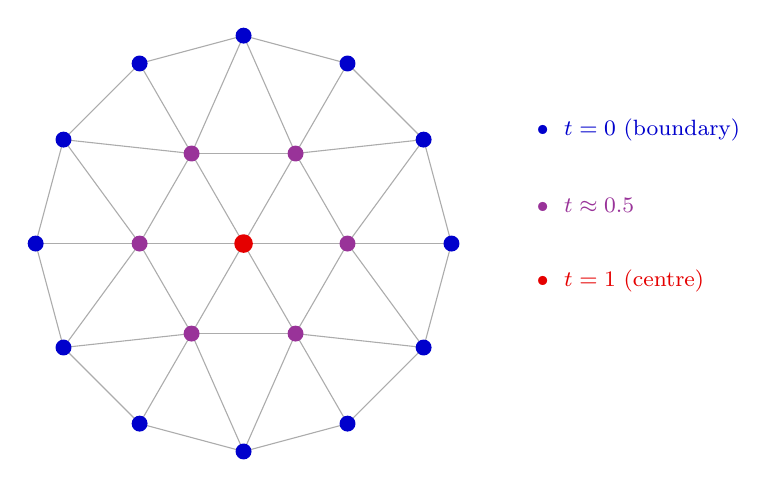
\begin{tikzpicture}[scale=1.2, line join=round]
        \pgfmathsetmacro{\Rb}{2.2}
        \pgfmathsetmacro{\Rm}{1.1}
        \foreach \i in {0,...,11} { \coordinate (b\i) at ({30*\i}:\Rb); }
        \foreach \i in {0,...,5}  { \coordinate (m\i) at ({60*\i}:\Rm); }
        \coordinate (ct) at (0, 0);
        \foreach \i in {0,...,11} {
            \pgfmathtruncatemacro{\next}{mod(\i+1, 12)}
            \draw[gray!65, thin] (b\i) -- (b\next);
        }
        \foreach \i in {0,...,5} {
            \pgfmathtruncatemacro{\next}{mod(\i+1, 6)}
            \draw[gray!65, thin] (m\i) -- (m\next);
        }
        \foreach \i in {0,...,5} { \draw[gray!65, thin] (ct) -- (m\i); }
        \foreach \i in {0,...,5} {
            \pgfmathtruncatemacro{\bal}{2*\i}
            \pgfmathtruncatemacro{\bnext}{mod(2*\i + 1, 12)}
            \pgfmathtruncatemacro{\bprev}{mod(2*\i + 11, 12)}
            \draw[gray!65, thin] (m\i) -- (b\bal);
            \draw[gray!65, thin] (m\i) -- (b\bnext);
            \draw[gray!65, thin] (m\i) -- (b\bprev);
        }
        \foreach \i in {0,...,11} { \fill[blue!80!black] (b\i) circle (2.4pt); }
        \foreach \i in {0,...,5}  { \fill[violet!80]      (m\i) circle (2.4pt); }
        \fill[red!90!black] (ct) circle (2.8pt);
        \node[blue!80!black, font=\footnotesize, right] at (3.0,  1.2) {$\bullet \ \ t = 0$ (boundary)};
        \node[violet!80,    font=\footnotesize, right] at (3.0,  0.4) {$\bullet \ \ t \approx 0.5$};
        \node[red!90!black, font=\footnotesize, right] at (3.0, -0.4) {$\bullet \ \ t = 1$ (centre)};
    \end{tikzpicture}
    \caption{Normalised geodesic distance $t$ on a triangulated patch.}
    \label{fig:dijkstra-distance}
\end{figure}

The weighting profile is
\begin{equation}
w(t) = \sqrt{2t - t^2}, \qquad t \in [0, 1]. \label{eq:profile}
\end{equation}
Geometrically, this is the height of the unit hemisphere as a function of horizontal offset, which is consistent with the spherical-cap assumption. The more important property is $w'(0) = +\infty$: the tangent is vertical at $t = 0$, so the patch tangent at the boundary is parallel to the tangent plane of the surrounding mesh, giving approximate $C^1$ continuity. A parabolic profile $4t(1-t)$ has $w'(0) = 4$ and produces a visible crease where the patch meets the surface. Figure~\ref{fig:profile-comparison} compares both.

\begin{figure}[H]
    \centering
    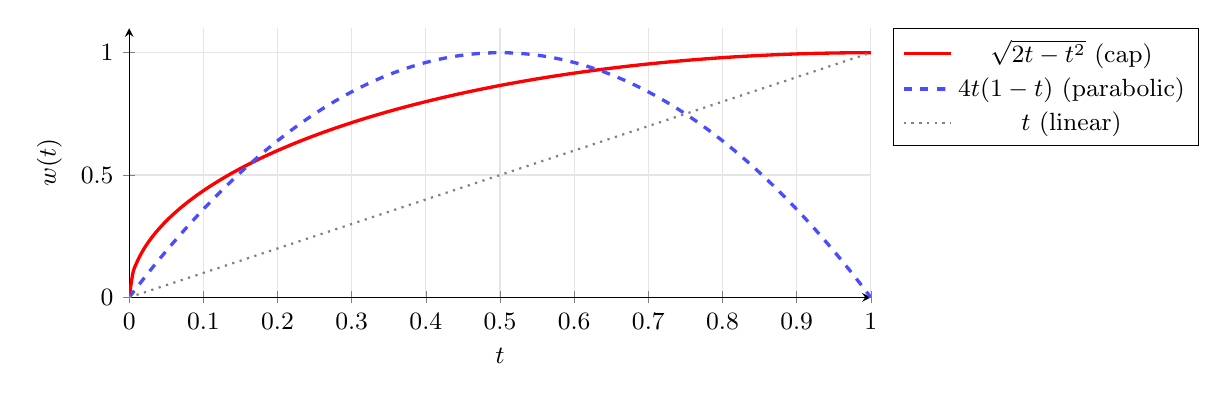
\begin{tikzpicture}
        \begin{axis}[
            width=11cm, height=5cm,
            xlabel={$t$}, ylabel={$w(t)$},
            domain=0:1, samples=200,
            xmin=0, xmax=1, ymin=0, ymax=1.1,
            axis lines=left, grid=both,
            grid style={gray!20, thin},
            legend pos=outer north east,
            legend style={font=\small},
            font=\small, no markers, smooth,
        ]
            \addplot[red, very thick] {sqrt(2*x - x*x)};
            \addlegendentry{$\sqrt{2t - t^2}$ (cap)}
            \addplot[blue!70, very thick, dashed] {4*x*(1 - x)};
            \addlegendentry{$4t(1-t)$ (parabolic)}
            \addplot[gray, thick, dotted] {x};
            \addlegendentry{$t$ (linear)}
        \end{axis}
    \end{tikzpicture}
    \caption{Displacement weighting profiles.}
    \label{fig:profile-comparison}
\end{figure}

The actual displacement is
\begin{equation}
v_i' = v_i + h \cdot w(t_i) \cdot \mathbf{n}_i^{\text{diff}},
\end{equation}
where the direction is the diffused normal from Stage~4, not the constant $\bar{\mathbf{n}}$. Using the spatially varying field allows the patch to bend differently on different sides, which matters on saddle-shaped boundaries.

After displacement, a few interior vertices may carry spike-like noise from irregular triangulation. Three pairs of Taubin smoothing ($\lambda = 0.40, \mu = -0.44$) clean this up: each pair is a positive (shrink) Laplacian step followed by a stronger negative (inflate) step. The combined filter attenuates high frequencies while preserving the dome.

\begin{figure}[H]
    \centering
    \begin{tikzpicture}[scale=1.0, line join=round, line cap=round]
        \pgfmathsetmacro{\L}{4.2}
        \pgfmathsetmacro{\H}{1.3}
        \begin{scope}[xshift=0cm]
            \draw[gray!70, thick] (0, 0) -- (\L, 0);
            \draw[red, thick, smooth, samples=180, domain=0:\L]
                plot (\x, {\H * sin(180*\x/\L)
                           + 0.22 * sin(180*14*\x/\L) * sin(180*\x/\L)});
            \fill[blue!80!black] (0, 0)  circle (2pt); \node[font=\footnotesize, below] at (0, 0)  {$\partial$};
            \fill[blue!80!black] (\L, 0) circle (2pt); \node[font=\footnotesize, below] at (\L, 0) {$\partial$};
            \node[font=\small\bfseries] at (\L/2, \H + 0.65) {Before Taubin};
        \end{scope}
        \draw[-{Stealth[length=3mm]}, very thick]
            (\L + 0.5, \H + 0.25) -- (\L + 1.6, \H + 0.25)
            node[midway, above, font=\small] {Taubin};
        \begin{scope}[xshift={\L + 2.2cm}]
            \draw[gray!70, thick] (0, 0) -- (\L, 0);
            \draw[red, thick, smooth, samples=120, domain=0:\L]
                plot (\x, {\H * sin(180*\x/\L)});
            \draw[green!50!black, dashed, thin]
                (0, \H) -- (\L, \H);
            \node[green!50!black, font=\footnotesize, right]
                at (\L, \H) {\ height preserved};
            \fill[blue!80!black] (0, 0)  circle (2pt); \node[font=\footnotesize, below] at (0, 0)  {$\partial$};
            \fill[blue!80!black] (\L, 0) circle (2pt); \node[font=\footnotesize, below] at (\L, 0) {$\partial$};
            \node[font=\small\bfseries] at (\L/2, \H + 0.65) {After Taubin};
        \end{scope}
    \end{tikzpicture}
    \caption{Taubin smoothing removes high-frequency spikes (left) without flattening the dome (right).}
    \label{fig:taubin-effect}
\end{figure}

\section{Patch merge}

The final stage stitches the patch into the host mesh. Boundary patch vertices are remapped to their original indices in $\mathcal{M}$ to avoid duplication. Interior patch vertices are appended with \texttt{AddVertices}, and faces are added with \texttt{AddFaces} after index translation. Vertex and face colours are averaged from boundary neighbours, so the patch does not appear as a white stripe on a coloured mesh. A final round of \texttt{UpdateTopology}, \texttt{UpdateNormal}, and \texttt{UpdateBounding} restores cached adjacency and attributes.
